% Options for packages loaded elsewhere
\PassOptionsToPackage{unicode}{hyperref}
\PassOptionsToPackage{hyphens}{url}
\PassOptionsToPackage{dvipsnames,svgnames,x11names}{xcolor}
%
\documentclass[
  letterpaper,
  DIV=11,
  numbers=noendperiod]{scrartcl}

\usepackage{amsmath,amssymb}
\usepackage{iftex}
\ifPDFTeX
  \usepackage[T1]{fontenc}
  \usepackage[utf8]{inputenc}
  \usepackage{textcomp} % provide euro and other symbols
\else % if luatex or xetex
  \usepackage{unicode-math}
  \defaultfontfeatures{Scale=MatchLowercase}
  \defaultfontfeatures[\rmfamily]{Ligatures=TeX,Scale=1}
\fi
\usepackage{lmodern}
\ifPDFTeX\else  
    % xetex/luatex font selection
\fi
% Use upquote if available, for straight quotes in verbatim environments
\IfFileExists{upquote.sty}{\usepackage{upquote}}{}
\IfFileExists{microtype.sty}{% use microtype if available
  \usepackage[]{microtype}
  \UseMicrotypeSet[protrusion]{basicmath} % disable protrusion for tt fonts
}{}
\makeatletter
\@ifundefined{KOMAClassName}{% if non-KOMA class
  \IfFileExists{parskip.sty}{%
    \usepackage{parskip}
  }{% else
    \setlength{\parindent}{0pt}
    \setlength{\parskip}{6pt plus 2pt minus 1pt}}
}{% if KOMA class
  \KOMAoptions{parskip=half}}
\makeatother
\usepackage{xcolor}
\setlength{\emergencystretch}{3em} % prevent overfull lines
\setcounter{secnumdepth}{-\maxdimen} % remove section numbering
% Make \paragraph and \subparagraph free-standing
\makeatletter
\ifx\paragraph\undefined\else
  \let\oldparagraph\paragraph
  \renewcommand{\paragraph}{
    \@ifstar
      \xxxParagraphStar
      \xxxParagraphNoStar
  }
  \newcommand{\xxxParagraphStar}[1]{\oldparagraph*{#1}\mbox{}}
  \newcommand{\xxxParagraphNoStar}[1]{\oldparagraph{#1}\mbox{}}
\fi
\ifx\subparagraph\undefined\else
  \let\oldsubparagraph\subparagraph
  \renewcommand{\subparagraph}{
    \@ifstar
      \xxxSubParagraphStar
      \xxxSubParagraphNoStar
  }
  \newcommand{\xxxSubParagraphStar}[1]{\oldsubparagraph*{#1}\mbox{}}
  \newcommand{\xxxSubParagraphNoStar}[1]{\oldsubparagraph{#1}\mbox{}}
\fi
\makeatother


\providecommand{\tightlist}{%
  \setlength{\itemsep}{0pt}\setlength{\parskip}{0pt}}\usepackage{longtable,booktabs,array}
\usepackage{calc} % for calculating minipage widths
% Correct order of tables after \paragraph or \subparagraph
\usepackage{etoolbox}
\makeatletter
\patchcmd\longtable{\par}{\if@noskipsec\mbox{}\fi\par}{}{}
\makeatother
% Allow footnotes in longtable head/foot
\IfFileExists{footnotehyper.sty}{\usepackage{footnotehyper}}{\usepackage{footnote}}
\makesavenoteenv{longtable}
\usepackage{graphicx}
\makeatletter
\def\maxwidth{\ifdim\Gin@nat@width>\linewidth\linewidth\else\Gin@nat@width\fi}
\def\maxheight{\ifdim\Gin@nat@height>\textheight\textheight\else\Gin@nat@height\fi}
\makeatother
% Scale images if necessary, so that they will not overflow the page
% margins by default, and it is still possible to overwrite the defaults
% using explicit options in \includegraphics[width, height, ...]{}
\setkeys{Gin}{width=\maxwidth,height=\maxheight,keepaspectratio}
% Set default figure placement to htbp
\makeatletter
\def\fps@figure{htbp}
\makeatother
% definitions for citeproc citations
\NewDocumentCommand\citeproctext{}{}
\NewDocumentCommand\citeproc{mm}{%
  \begingroup\def\citeproctext{#2}\cite{#1}\endgroup}
\makeatletter
 % allow citations to break across lines
 \let\@cite@ofmt\@firstofone
 % avoid brackets around text for \cite:
 \def\@biblabel#1{}
 \def\@cite#1#2{{#1\if@tempswa , #2\fi}}
\makeatother
\newlength{\cslhangindent}
\setlength{\cslhangindent}{1.5em}
\newlength{\csllabelwidth}
\setlength{\csllabelwidth}{3em}
\newenvironment{CSLReferences}[2] % #1 hanging-indent, #2 entry-spacing
 {\begin{list}{}{%
  \setlength{\itemindent}{0pt}
  \setlength{\leftmargin}{0pt}
  \setlength{\parsep}{0pt}
  % turn on hanging indent if param 1 is 1
  \ifodd #1
   \setlength{\leftmargin}{\cslhangindent}
   \setlength{\itemindent}{-1\cslhangindent}
  \fi
  % set entry spacing
  \setlength{\itemsep}{#2\baselineskip}}}
 {\end{list}}
\usepackage{calc}
\newcommand{\CSLBlock}[1]{\hfill\break\parbox[t]{\linewidth}{\strut\ignorespaces#1\strut}}
\newcommand{\CSLLeftMargin}[1]{\parbox[t]{\csllabelwidth}{\strut#1\strut}}
\newcommand{\CSLRightInline}[1]{\parbox[t]{\linewidth - \csllabelwidth}{\strut#1\strut}}
\newcommand{\CSLIndent}[1]{\hspace{\cslhangindent}#1}

\KOMAoption{captions}{tableheading}
\makeatletter
\@ifpackageloaded{caption}{}{\usepackage{caption}}
\AtBeginDocument{%
\ifdefined\contentsname
  \renewcommand*\contentsname{Table of contents}
\else
  \newcommand\contentsname{Table of contents}
\fi
\ifdefined\listfigurename
  \renewcommand*\listfigurename{List of Figures}
\else
  \newcommand\listfigurename{List of Figures}
\fi
\ifdefined\listtablename
  \renewcommand*\listtablename{List of Tables}
\else
  \newcommand\listtablename{List of Tables}
\fi
\ifdefined\figurename
  \renewcommand*\figurename{Figure}
\else
  \newcommand\figurename{Figure}
\fi
\ifdefined\tablename
  \renewcommand*\tablename{Table}
\else
  \newcommand\tablename{Table}
\fi
}
\@ifpackageloaded{float}{}{\usepackage{float}}
\floatstyle{ruled}
\@ifundefined{c@chapter}{\newfloat{codelisting}{h}{lop}}{\newfloat{codelisting}{h}{lop}[chapter]}
\floatname{codelisting}{Listing}
\newcommand*\listoflistings{\listof{codelisting}{List of Listings}}
\makeatother
\makeatletter
\makeatother
\makeatletter
\@ifpackageloaded{caption}{}{\usepackage{caption}}
\@ifpackageloaded{subcaption}{}{\usepackage{subcaption}}
\makeatother

\ifLuaTeX
  \usepackage{selnolig}  % disable illegal ligatures
\fi
\usepackage{bookmark}

\IfFileExists{xurl.sty}{\usepackage{xurl}}{} % add URL line breaks if available
\urlstyle{same} % disable monospaced font for URLs
\hypersetup{
  pdftitle={hw\_6},
  colorlinks=true,
  linkcolor={blue},
  filecolor={Maroon},
  citecolor={Blue},
  urlcolor={Blue},
  pdfcreator={LaTeX via pandoc}}


\title{hw\_6}
\author{}
\date{}

\begin{document}
\maketitle


\subsection{Commit 1}\label{commit-1}

\paragraph{Load libraries}\label{load-libraries}

\begin{verbatim}
-- Attaching core tidyverse packages ------------------------ tidyverse 2.0.0 --
v dplyr     1.1.4     v readr     2.1.5
v forcats   1.0.0     v stringr   1.5.1
v ggplot2   3.5.1     v tibble    3.2.1
v lubridate 1.9.3     v tidyr     1.3.1
v purrr     1.0.2     
-- Conflicts ------------------------------------------ tidyverse_conflicts() --
x dplyr::filter() masks stats::filter()
x dplyr::lag()    masks stats::lag()
i Use the conflicted package (<http://conflicted.r-lib.org/>) to force all conflicts to become errors

Attaching package: 'janitor'


The following objects are masked from 'package:stats':

    chisq.test, fisher.test


here() starts at C:/Users/forrest/OneDrive/Documents/EDLD_651/homework_6/hw_6
\end{verbatim}

\paragraph{Code to load data}\label{code-to-load-data}

\begin{verbatim}
  schidkn  sex frl reg_size reg_size_aid small_size white black other totexp
1      63 girl  no        0            0          1     1     0     0      7
2      20 girl  no        0            0          1     0     1     0     21
3      19  boy yes        0            1          0     0     1     0      0
4      69  boy  no        1            0          0     1     0     0     16
5      79  boy yes        0            0          1     1     0     0      5
6       5  boy yes        1            0          0     1     0     0      8
  tmathss treadss
1     473     447
2     536     450
3     463     439
4     559     448
5     489     447
6     454     431
\end{verbatim}

\subsubsection{Commit 2}\label{commit-2}

Today's group meeting discussed the following. 1. Group by ID, select ID
response time Nabi, Gustafson, and Jensen (2018). For Scatter plot. what
questions should we ask? Example: What is the relationship between error
and response time? (Cabán et al. 2023; Thompson and Ofori-Parku 2021).
What is the position of the cycle and the relationship from that to the
response time?

\subsubsection{\texorpdfstring{\textbf{Commit
3}}{Commit 3}}\label{commit-3}

\begin{enumerate}
\def\labelenumi{\arabic{enumi}.}
\tightlist
\item
  Write the code to create the summary statistics shown in the table
  below. Output the table below and briefly describe it in text.
\end{enumerate}

\subsubsection{Commit 4}\label{commit-4}

Create the following plot, using whatever theme you'd like, and briefly
discuss it in text. (Note that might need to problem-solve how to put
the legend at the bottom.)

A: got everything to be similar aside from the difference in color of
FRL yes and no, but this says basically the same thing. We see that
there isn't a huge difference in math scores based on number of teachers
experience until you get to around 24 years of experience, there is no
longer a math score under 423. However since there are only two teachers
above 24 years of teaching experience compared with under 24, I wouldn't
hold too much weight in this observation. As with the FRL lines, we see
that when kids receive FRL, they tend to have lower math scores on
average then kids who pay for lunch regardless of their respective
teachers experience.

\begin{verbatim}
`geom_smooth()` using formula = 'y ~ x'
\end{verbatim}

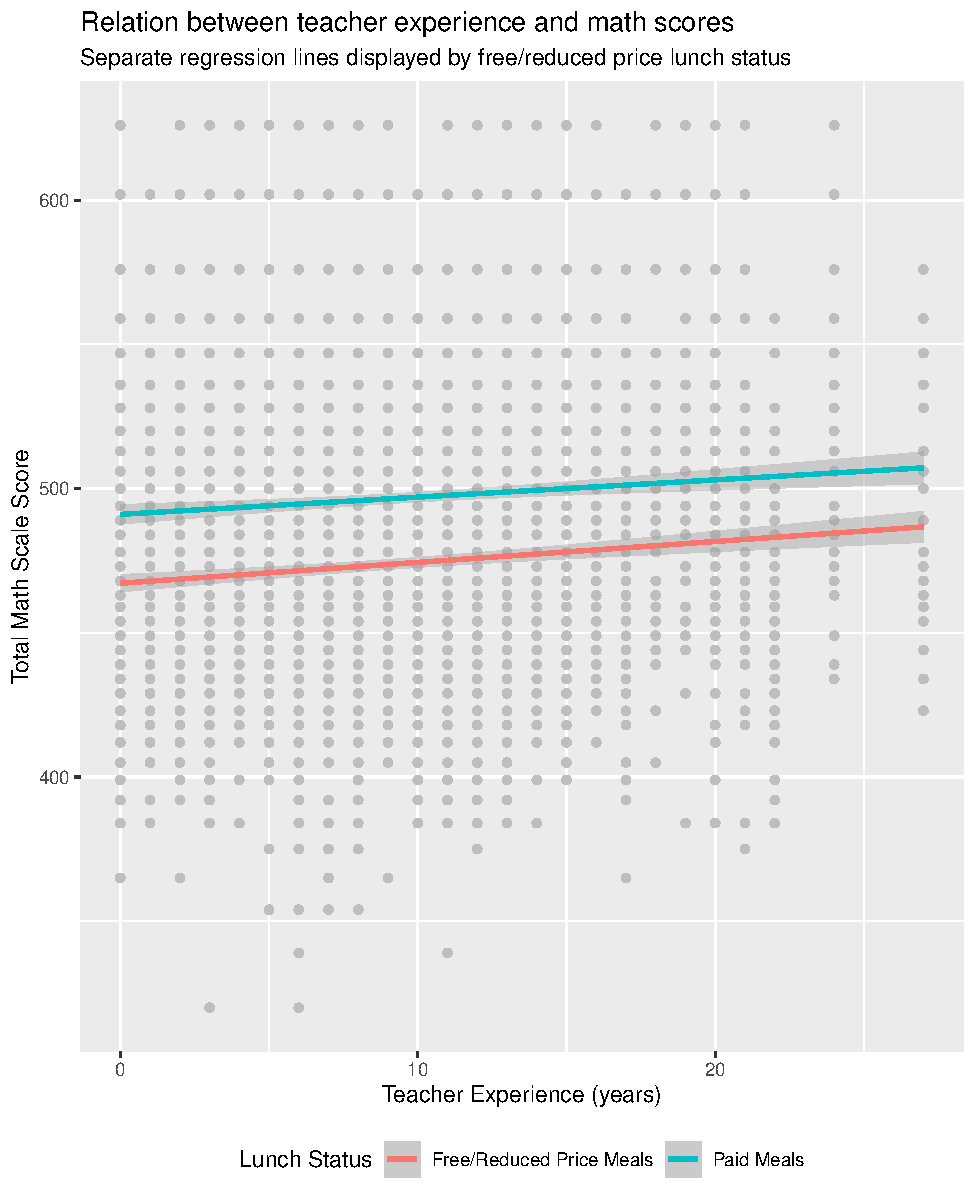
\includegraphics{hw_6_files/figure-pdf/unnamed-chunk-3-1.pdf}

\section*{References}\label{references}
\addcontentsline{toc}{section}{References}

\phantomsection\label{refs}
\begin{CSLReferences}{1}{0}
\bibitem[\citeproctext]{ref-cabuxe1n2023}
Cabán, Madelyn, Justas V. Rodarte, Madeleine Bibby, Matthew D. Gray,
Justin J. Taylor, Marie Pancera, and Jim Boonyaratanakornkit. 2023.
{``Cross-Protective Antibodies Against Common Endemic Respiratory
Viruses.''} \emph{Nature Communications} 14 (1): 798.
\url{https://doi.org/10.1038/s41467-023-36459-3}.

\bibitem[\citeproctext]{ref-nabi2018}
Nabi, Robin L., Abel Gustafson, and Risa Jensen. 2018. {``Framing
Climate Change: Exploring the Role of Emotion in Generating Advocacy
Behavior.''} \emph{Science Communication} 40 (4): 442--68.
\url{https://doi.org/10.1177/1075547018776019}.

\bibitem[\citeproctext]{ref-thompson2021}
Thompson, Esi E., and S. Senyo Ofori-Parku. 2021. {``Advocacy and
Mobilizing for Health Policy Change: Ghanaian News Media{'}s Framing of
a Prescription Opioid Crisis.''} \emph{Health Communication} 36 (14):
1909--20. \url{https://doi.org/10.1080/10410236.2020.1808403}.

\end{CSLReferences}




\end{document}
